\section{An introduction to Bayesian workflow}

The idea of statistical workflow is not new.
One early example of a statistical workflow can be found in% \cite{box_science_1976}.
In the Bayesian context, \cite{gabry_visualization_2019} and \cite{betancourt_towards_2020} have referred to the idea of a Bayesian workflow.
This section summarizes the ideas behind Bayesian workflow as presented by \cite{gelman_bayesian_2020}.

While Bayesian \textit{inference} deals with the formulation and computation of (conditional) probability densities, Bayesian \textit{workflow} consists of three steps: model building, inference and model checking/improvement.
In Bayesian workflow, it is inevitable to fit a series of models iteratively.
Flawed models are a necessary step towards improving the model and finding models that are useful in practice.
At the same time, model improvement is not limited to finding the best model, but it also allows to better understand the models used; specifically, why they fail or lead to different results under certain conditions.
There are several reasons for considering a workflow and not just plain inference.
Bayesian computation is challenging and it is often necessary to iterate through simpler and alternative models, sometimes using faster but less precise approximation algorithms.
Moreover, it might not be clear ahead of time which model adequate and how it can be modified or extended.
The relation between fitted models and data can be best understood by comparing inferences from different models.
For example, it is possible to gain valuable insights by comparing a model to simpler or more complex models.
Finally, there is uncertainty associated with model choice, as different models might display diverging but realistic results for the same application.

The graphical representation of the workflow is included in Figure \ref{fig:gelman_wf}.
The workflow contains many steps, but the authors emphasize that there are some steps that might be skipped or changed depending on the data and the use case.
For this reason, \cite{gelman_bayesian_2020} argues that a workflow is more general than an example, but less clearly specified than a methodology.
While the exact steps are likely to vary depending on the specific application, a workflow provides a framework to develop statistical models.
Note that this workflow is mostly focused on data modeling.
Other steps such as data collection are not taken into account.

\begin{figure}
    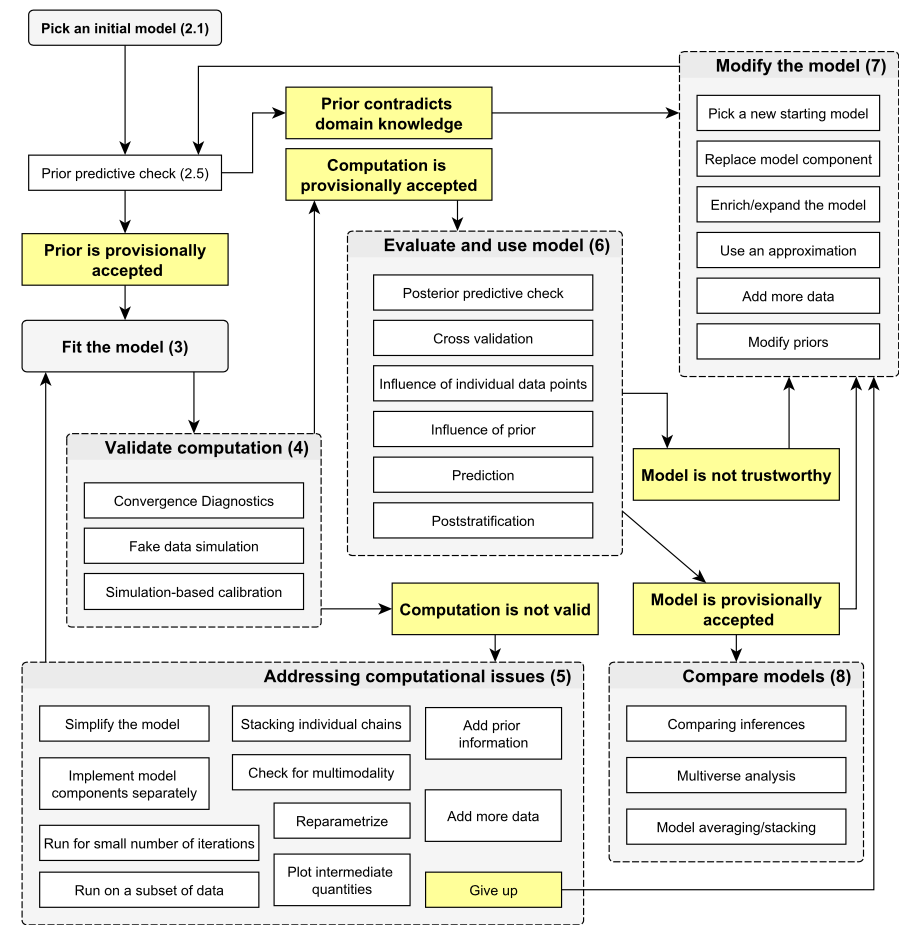
\includegraphics[width=16cm]{./graphics/workflow}
    \label{fig:gelman_wf}
    \caption{Workflow from Gelman et al. (2020).}
\end{figure}


An exhaustive discussion of the whole workflow is beyond the scope of the present paper.
Instead, the focus is on how the ideas in \cite{gelman_bayesian_2020} can be applied to the estimation of poverty indicators in the small area estimation context.
Due to the non-linear nature of the workflow, the sections and subsections in the current chapter are not strictly named after single steps of the workflow.
On the contrary, each section in this chapter reflect specific aspects of a model that are investigated separately.
However, throughout the rest of the paper there are explicit references to the corresponding step and an explanation of why it is necessary at a given stage.
For completeness, the rest of this section summarizes the seven workflow steps in \cite{gelman_bayesian_2020} that are also represented in Figure \ref{fig:gelman_wf}.

\subsection{Step 1. Pick an initial model}

Usually, the starting point is to adapt an idea that already exists in the literature.
This adaptation can be done in different ways: (i) start with a simple model and add layers of complexity, (ii) simplify a complex model, so that it is more understandable or easier to fit while still delivering a similar performance, (iii) consider different starting models with diverging assumptions and follow multiple paths.
Bayesian models are highly modular, as priors and likelihood can be replaced with other distributions if necessary.
Moreover, there is flexibility regarding how parameter priors interact with each other, which allows for a high degree of model complexity.

%(HERE? )Prior predictive checks are a valuable tool when building a model, because it allows to refine the model without fitting the data multiple times.
%This is especially important when the priors should regularize the model to avoid extreme predictions.
%Additionally, fully generative model?

Here, the initial model is the HB model by \cite{molina_small_2014} with its extensions in \cite{morelli_hierarchical_2021}, where the effect of different likelihoods for log-shift transformed income was explored.
The $t$-distribution provides the best performance over many different scenarios.
However, in \cite{morelli_hierarchical_2021} the shift parameter was found through a heuristic whereas
the initial model in the present paper does full inference on the shift parameter from the start.
Additionally, an alternative group of initial models that use skewed likelihoods instead of transformation will be considered in section \ref{ch:skewed_likelihoods}.


\subsection{Step 2. Fit the model}

Appendix \ref{ch:computation} discusses the two most common Bayesian estimation approaches: MCMC and variational inference.
When fitting a model, the user is confronted with decisions on which algorithm to run and under which conditions.
To make an adequate choice, it is necessary to be aware of the modelling stage.
MCMC provides the most exact approximation, which becomes more robust with more samples and more chains.
However, if a model was just modified or the user is at an early stage of model development, it is not efficient to fit the model the most exact algorithms and a high number of samples with multiple chain.
Instead, the fit of a bad model should fail fast, as computational issues usually indicate a deeper problem in the model.
Such problems can already be clear with just two Markov chain and a drastically lower number of sample than would be taken for the final model.
Even a check with an approximate method such as variational inference might be enough to notice problems with the model, while being drastically faster than MCMC.
In this paper, variational algorithms were often used to do a first fit of the model.
(CHECK AGAIN) While iterating through the models only 2 Markov chains were used and, depending on fitting time, the number of iterations was reduced compared to the default in \code{Stan}.


\subsection{Step 3. Validate computation}

Diagnostics for Bayesian computation methods are discussed in detail in appendix \ref{ch:computation}.
When using an MCMC algorithm such as NUTS, the two main aims are to have no divergences and to have an $\hat R$ lower than 1.01.
All the models presented in this paper fulfill at least these two conditions, unless otherwise specified.
However, adequate diagnostic values are a necessary but not sufficient condition for a reliable model.
To assess model quality, it has to be fitted to some data set.
The use of real data can be challenging, as there is no way to distinguish modeling issues from computational issues.
This problem can be avoided by using simulated data, ideally from multiple realistic scenarios.
Section \ref{ch:simulations}, already presented three scenarios used in this paper.
A model that can fit fake data, is not necessarily correct, but a model that fails when fitting simulating data will also fail with real data.
This paper deals primarily with prediction, so it is enough if samples from the posterior predictive distribution capture the main characteristics of the data.
There will be less emphasis on correctly recovering model parameters from the simulated data.

%(Another approach with simulated data is simulation-based calibration.
%First, model parameters are generated from the prior and used to simulate data conditional on these values.
%Then the model is fitted to data and the posterior is compared to the simulated parameters from the priors that were used to generate the data.
%By repeating this procedure, it is possible to check the inference algorithms – the prior should be recovered when performing inference on data sets drawn from the prior.)

\subsection{Step 4. Address computational issues}

A model that leads to computational problems usually has some underlying modelling issues.
Usually, it is best to start with a simple model and make it more complex one step at a time, making it easier to determine what part of the model is causing problems.
On the other hand, if the model is already complex and shows signs of computational problems, then it is useful to simplify it step by step until the computation is successful.
For example, in a model with numerous groups of random intercepts or random slopes it makes sense to start with just one group and then add each additional group one step at a time, so as to know whether the estimation is working.
A common source of computational problems is prior choice.
Tightening moderately informative priors can help by pushing the sampler towards certain regions of the parameter space.
However, this adjustment of priors should be in line with available knowledge and not only to solve fitting problems.
One such example is discussed in section \ref{ch:log_shift}.

\subsection{Step 5. Evaluate and use the model}

Posterior predictive checks are a useful tool when diagnosing fitting problems to the data.
This can be seen as a safeguard against misspecification.
Moreover, such checks might reveal which aspects of the data are not captured well by the model.
Cross-validation is an alternative to posterior predictive checks and has the advantage that part of the data is left out.
Thus, it is less optimistic than posterior predictive checks, which uses the data for both model fitting and evaluation.
While refittig model multiple times to do cross-validation can be computationally expensive, there are efficients approximations such as PSIS-LOO \citep{vehtari_practical_2017}.
To check how informative the data is with respect to a parameter, one can compare the standard deviation of prior and posterior parameters. A higher shrinkage in uncertainty indicates that the data is more informative.

\subsection{Step 6. Modify the model}

Bayesian statistics provides a modular approach in which models can be expanded or reduced in response to new data or failures to fit the model to the data.
This is usually done by changing certain aspects of the prior distribution.
The prior determines what kind of available information is integrated into the model and acts as a constraint on the fitting procedure.
There are various levels of priors from completely non-informative to highly informative.
However, the way prior information acts on this information depends on the type of parameter.
Parameters controlling central quantities like a mean are less sensitive to weak priors than scale parameters such as variance.
In turn, scale parameters are less sensitive to weak priors than shape parameters, which control the tails of a distribution (e.g., the degrees of freedom in a $t$-distribution).
When expanding the model with additional parameters (e.g., introducing random intercepts or random slopes), it should be considered whether the priors should be tightened to stabilize the estimates, as the amount of data has not changed.
Nevertheless, the priors should not be tightened beyond a range compatible with prior information.

\subsection{Step 7. Compare models}

Models are fitted many times, for multiple reasons.
It might be easier to start with simple models, before getting to a more complex model. There are often bugs in the code and in the models.
A model might be well-specified, but it could be improved by expanding it.
The priors might be only placeholders, which will be replaced at a later stage.
Moreover, multiple model might provide acceptable results.

Comparing different models is always tied to a certain degree of uncertainty.
Instead of choosing the model with the best cross-validation results, using model stacking can give an insight into model differences.
Stacking combines inferences using a weighting that minimizes cross-validation error .
Roughly speaking, if a model outperforms another model 80\% of the time, the weights will be 0.8 for the first model and 0.2 for the second model.
This is an indication of model heterogeneity, which can be used as a guide to improve the model \citep{yao_using_2018}.
Thus, stacking is not limited to combinining predictions from different models.
At the same time, care must be taken when comparing a large number of models to reduce the risk of overfitting.
Therefore, it is useful to select only a couple of models at each stage of the workflow for a comparison.
